\section{Coordinate Systems and Frames of Reference}

\subsection{Inertial Frame of Reference}
The inertial reference frame is defined as a coordinate system that is not accelerating or rotating. Typically, the earth is chosen to be the inertial reference frame of the vehicle.


\subsection{Euler Angles}

Euler Angles are a series of sequential rotations for a given coordinate system. This formulation is commonly used to convert between different coordinate systems. \newline

The most common symbols for \textbf{Euler Angles} in aircraft dynamics are $\theta$ (pitch), $\psi$(yaw), $\phi$(rolls)

 \begin{figure}[h]
    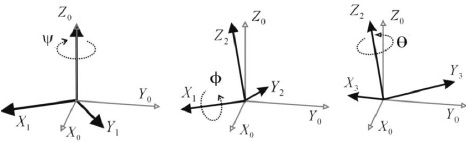
\includegraphics[width=10cm]{euler_frames}
    \centering
    \label{fig:euler_angles}
    \caption{Sequential Rotations of Euler Angles}
\end{figure}

\subsubsection{Euler Rotation Matrix}

By using trigonometry, between each pair of coordinates above it is possible to show that rotations between frames can be expressed as the product of elementary rotation matrices obtained from each rotation about intermediate axes. 

$$
R_{x}(\phi) = \begin{bmatrix}
    1 & 0 & 0\\ 
    0 & c(\phi) & -s(\phi)\\
    0 & s(\phi) & c(\phi)
\end{bmatrix} \quad
R_{y}(\theta) = \begin{bmatrix}
    c(\theta) & 0 & s(\theta)\\
    0 & 1 & 0\\
    -s(\theta) & 0 & \c(\theta)
\end{bmatrix} \quad
R_{z}(\psi) = \begin{bmatrix}
    c(\psi) & -s(\psi) & 0\\
    s(\psi) & c(\psi) & 0\\
    0 & 0 & 1
\end{bmatrix}  $$ 

These elementary rotation matrices can be combined to to produce a single rotation matrix. 

$$ R_{zyx}(\phi, \theta, \psi)\biggr\rvert_{B}^{I} = R_{x}(\phi) \cdot R_{y}(\theta) \cdot R_{z}(\psi)$$

$$ R_{zyx}(\phi, \theta, \psi)\biggr\rvert_{B}^{I} = \begin{bmatrix}
    c(\theta)c(\psi) & s(\phi)s(\theta)c(\psi)-c(\phi)s(\psi) & c(\phi)s(\theta)c(\psi)+s(\theta)s(\psi)\\
    c(\theta)s(\psi) & s(\phi)s(\theta)s(\psi)+c(\phi)c(\psi) & c(\phi)s(\theta)s(\psi)-s(\theta)c(\psi)\\
    -s(\theta) & s(\phi)c(\theta) & c(\phi)c(\theta)
\end{bmatrix}$$

It should also be noted that since this rotation matrix is orthogonal, it's inverse can be found by taking the transpose... 

$$ R^{-1} = R^{T}$$

\subsubsection{Euler Rates to Angular Velocity Components (\& Vise Versa)}

$$ T(\phi, \theta, \psi) = \begin{bmatrix}
    1 & s(\phi)t(\theta) & c(\phi)t(\theta)\\
    0 & c(\phi) & -s(\phi)\\
    0 & \frac{s(\phi)}{c(\theta)} & \frac{c(\phi)}{c(\theta)}
\end{bmatrix}$$



$$\bvectdot{x}{y}{x} = R(\phi, \theta, \psi) \cdot \bvect{u}{v}{w} \quad , \quad  \bvectdot{\phi}{\theta}{\psi} = T(\phi, \theta, \psi) \cdot \bvect{p}{q}{r} $$

It should be noted that the body frame angular velocities are not equal to the Euler rates. This is due to the fact that the angular velocity components exist simultaneously as components of the angular velocity vector $\vect{\omega}$. However, Euler angles do not exist at the same time, they constitute a sequence of three consecutive rotations around different axes of rotations. 



$$\bvectdot{p}{q}{r} = \bvect{\dot{\phi}}{0}{0} + R() \bvect{0}{\dot{\theta}}{0} + R()R() \bvect{0}{0}{\dot{\psi}}$$

These transformations convert between the angular velocity and the euler rates (and vise versa)

$$ \bvect{p}{q}{r} = \begin{bmatrix}
    1 & 0 & -s(\theta)\\
    0 & c(\phi) & s(\phi)c(\theta)\\
    0 & -s(\phi) & c(\phi)c(\theta) \end{bmatrix}  \bvectdot{\phi}{\theta}{\psi}$$

$$ \bvectdot{\phi}{\theta}{\psi} = \begin{bmatrix}
    1 & s(\phi)t(\theta) & c(\phi)t(\theta)\\
    0 & c(\phi) & -s(\phi)\\
    0 & \frac{s(\phi)}{c(\theta)} & \frac{c(\phi)}{c(\theta)} \end{bmatrix} \bvect{p}{q}{r} $$

\subsubsection{Problem with Euler Angles}
The main drawback of using Euler angles is the presence of gimbal lock where there does not exist a unique mathematical description of the orientation given the angles. 

\subsection{Quaternions}
The most commonly used alternative to Euler angles is the quaternion formulation. 

$$ 
q = q_{0} + q_{1}\hat{i} + q_{2}\hat{j} + q_{3}\hat{k} 
$$
$$q = \begin{bmatrix}
    q_0  & q_1 &  q_2 & q_3
\end{bmatrix}^{T}$$

\subsubsection{Quaternion Properties}

The product of two quaternions is defined as the Kronecker product as defined below.

$$p \times q = \begin{bmatrix}
    p_0q_0 - p_1q_1 - p_2q_2 - p_3q_3 \\
    p_0q_1 + p_1q_0 + p_2q_3 - p_3q_2 \\
    p_0q_2 - p_1q_3 + p_2q_0 + p_3q_1 \\
    p_0q_3 + p_1q_2 - p_2q_1 + p_3q_0
\end{bmatrix}$$


A quaternion can be represented as a $4x4$ matrix given $q = [q_0, q_1, q_2, q_3]$... 

$$\begin{bmatrix}
    q_0 & -q_1 & -q_2 & -q_3 \\
    q_1 & q_0 & -q_3 & q_2 \\
    q_2 & q_3 & q_0 & -q_1 \\
    q_3 & -q_2 & q_1 & q_0
\end{bmatrix}$$

Quaternion multiplication can be cast into a Matrix vector product by using this expansion of the quaternion into a matrix 

$$R = q \otimes p = \begin{bmatrix}
    q_0 & -q_1 & -q_2 & -q_3 \\
    q_1 & q_0 & -q_3 & q_2 \\
    q_2 & q_3 & q_0 & -q_1 \\
    q_3 & -q_2 & q_1 & q_0
\end{bmatrix} \begin{bmatrix}
    p_0 \\
    p_1\\
    p_2 \\
    p_3
\end{bmatrix}$$




Or if desired, can be expressed as matrix multiplication 

$$p \times q = Q(p)q = \begin{bmatrix}
    p_0 & -p_1 & -p_2 & -p_3 \\
    p_1 & p_0 & -p_3 & p_2 \\
    p_2 & p_3 & p_0 & -p_1 \\
    p_3 & -p_2 & p_1 & p_0 
\end{bmatrix} \begin{bmatrix}
    q_0 \\ q_1 \\ q_2 \\ q_3
\end{bmatrix}$$

The conjugate of a quaternion is simply the negated vector components of the quaternion. 

$$q^{*} = \begin{bmatrix}
    q_0 & -q_1 & -q_2 & -q_3
\end{bmatrix}$$ 

One of the most important properties that needs to be known for simulations that use quaternions is how to define the derivative of a quaternion so that an update law can be defined. 

$$\dot{q_{\omega}(q, \omega) = \frac{1}{2}q\times\begin{bmatrix} 
    0 \\ 
    \omega
\end{bmatrix} = \frac{1}{2}Q(q)\times\begin{bmatrix} 
    0 \\ 
    \omega
\end{bmatrix} 
    $$

\subsubsection{Using the Quaterion}
$$w = q\times \begin{bmatrix}
    0 \\ v
\end{bmatrix}\times q^{*}$$

\subsection{Quaternion Rotation Matrix}
Quaternions can be used as a drop-in replacement for Euler-angles by the use of a quaternion based rotation matrix. 

$$R_{i}^{b}({q_{i}^{b}}) = \begin{bmatrix}
    {q_0}^{2}+ {q_1}^{2} - {q_2}^{2} - {q_3}^{2} & 2(q_{1}q_{2}) - 2(q_{0}q_{3}) & 2(q_{1}q_{3}) - 2(q_{0}q_{2})\\
    2(q_{1}q_{2}) + 2(q_{0}q_{3}) & {q_0}^{2}- {q_1}^{2} + {q_2}^{2} - {q_3}^{2} &  2(q_{2}q_{3}) - 2(q_{0}q_{1})\\
    2(q_{1}q_{3}) - 2(q_{0}q_{3}) & 2(q_{2}q_{3}) + 2(q_{0}q_{1}) & {q_0}^{2}- {q_1}^{2} - {q_2}^{2} + {q_3}^{2}
    \end{bmatrix}$$ 

However, this usage is computationally inefficient compared to direct conversion using quaternion multiplication directly, which is the preferred method of computing transformations.

\subsection{Derivatives of Quaternions}
Like Euler rates relate to Euler Angles, it is necessary to be able to define and compute the derivatives of quaternions as these process allows for us to evolve and align the quaternion in time with the body frame of the quadcopter.

\subsubection{Angular Velocity based Quaternion Derivatives}

Direct derivatives can be computed using the angular velocity of the system. 

$$\dot{q} = \frac{1}{2}q
\otimes \begin{bmatrix}
    0 \\ 
    \omega
\end{bmatrix}$$

Expanded this shows... 

$$\begin{bmatrix}
   \dot{q_{0}} \\
   \dot{q_{1}} \\
   \dot{q_{2}} \\
   \dot{q_{3}} \\  
\end{bmatrix} = \frac{1}{2}\begin{bmatrix}
    0 & -p & -q & -r \\
    p & 0 & r & -q \\
    q & -r & 0 & p  \\
    r & q & -p & 0 
    
\end{bmatrix}\begin{bmatrix}
    q_{0} \\
    q_{1} \\
    q_{2} \\
    q_{3} 
 \end{bmatrix} $$

\subsubsection{Numerical methods }


\subsection{Numerical Integration of Quaternions}

\subsubsection{Digital Integration of Quaternions}

$$q_{k+1} = q_{k} + \int_{t_{k+1}}^{t_k} \frac{d}{dt}q(\tau) \,d\tau $$

\subsection{Quaternion Normalization for Numerical Methods}

Unlike Euler-Rates, in order for quaternions to retain some of their desireable properties, they must be normalized to 1. Therefore, for either method of computing the quaternion derivative above, numerical errors will build up and begin to diverge the norm of the quaternion from unity. Therefore a robust numerical implementation of the quaternion derivatives requires periodic normalization. \\

The most simple way of accomplishing this is by brute-force normalizing the quaternion after every time-step in the update law. 

$$q _{k+1} \rightarrow \frac{q_{k+1}}{\norm{q_{k+1}}}$$

\subsubsection{Runge-Kutta Integration of Quaternions}

$$f(q,t) = \frac{1}{2}\Omega(\omega(t))q$$

$$q_{k+1} = q_k + \deltat \sum_{i=1}^{s}b_{i}k^{(i)}$$ 

$$k^{(i)} = f(q^{(i), t_k + c_{i}\delta t})$$

$$q^{(i)} = q_k + \delta \sum_{j=1}^{i-1}a_{ij}k^{(j)}$$